% BeyondNN -- TNNLS revision (reconstructed manuscript).
% This LaTeX source was RECONSTRUCTED for the TNNLS revision on 2026-11-03 from (i) the text of
% the 16-page TNNLS PDF supplied by the authors (SHA-256 0471417f...a1fa60; no LaTeX source of
% that version was available) and (ii) verified repository evidence. It is not the original
% source. See docs/tnnls_revision/MANUSCRIPT_CHANGELOG.md.
\documentclass[journal]{IEEEtran}
\usepackage{amsmath,amssymb,amsthm}
\usepackage{graphicx}
\usepackage{booktabs}
\usepackage{multirow}
\usepackage[hidelinks]{hyperref}
\usepackage{xurl}
\usepackage{cite}
\usepackage{tikz}
\usetikzlibrary{positioning,arrows.meta,fit,calc}
\newtheorem{definition}{Definition}
\newtheorem{proposition}{Proposition}

% generated by make_tables.py -- do not edit
\newcommand{\BOneLoc}{54}
\newcommand{\CnnFixed}{10}
\newcommand{\CnnHidFixed}{1}
\newcommand{\CnnHidKOnly}{0}
\newcommand{\CnnHidRev}{1}
\newcommand{\CnnHidSup}{1}
\newcommand{\CnnKOnly}{3}
\newcommand{\CnnRev}{13}
\newcommand{\CnnSup}{14}
\newcommand{\CostBnnMs}{55.3}
\newcommand{\CostPlainMs}{2.38}
\newcommand{\CostRatio}{23}
\newcommand{\IbFp}{18}
\newcommand{\IbFpPct}{0.20}
\newcommand{\IbNeg}{8858}
\newcommand{\IbPos}{942}
\newcommand{\IbTp}{942}
\newcommand{\IbZeroFp}{1155}
\newcommand{\IbZeroFpPct}{13.0}
\newcommand{\MlpFixed}{3}
\newcommand{\MlpHidFixed}{2}
\newcommand{\MlpHidKOnly}{0}
\newcommand{\MlpHidRev}{2}
\newcommand{\MlpHidSup}{4}
\newcommand{\MlpKOnly}{4}
\newcommand{\MlpRev}{7}
\newcommand{\MlpSup}{8}
\newcommand{\PlanLoc}{98}
\newcommand{\ReproDiffs}{0}
\newcommand{\TinyFixed}{3}
\newcommand{\TinyKOnly}{10}
\newcommand{\TinyRev}{13}
\newcommand{\TinySup}{14}
\newcommand{\TotFixed}{19}
\newcommand{\TotKOnly}{17}
\newcommand{\TotKSingle}{26}
\newcommand{\TotNotRev}{5}
\newcommand{\TotNull}{11}
\newcommand{\TotRepl}{15}
\newcommand{\TotRev}{36}
\newcommand{\TotSup}{41}
\newcommand{\TotThr}{0}

\begin{document}

\title{BeyondNN: Auditing Interpretability Claims about Neural Networks with Provenance, Controls, and Counterevidence}

\author{Nikolaos~Roufas and Andreas~Kanavos
\thanks{N. Roufas and A. Kanavos are with the Department of Informatics, Ionian University, Corfu, Greece (e-mail: inf2024146@ionio.gr; akanavos@ionio.gr).}}

\markboth{IEEE Transactions on Neural Networks and Learning Systems}{Roufas and Kanavos: BeyondNN}

\maketitle

\begin{abstract}
Interpretability methods produce measurements, but a measurement does not by itself establish the claim commonly attached to it. We present BeyondNN, an evidence and audit layer for PyTorch that records typed, provenance-bound evidence, represents claims about neural networks by relation, subject, scope and eligible units, and re-derives each claim's standing under declared \textsc{primary}, \textsc{alternative} and \textsc{stress\_test} configurations. We give a formal semantics for evidence admissibility, test outcomes and standings, with six properties that hold by construction. On six held-out sites of trained MLP, CNN, BERT-tiny and BERT-base models, 47 of 52 \textsc{primary}-supported Integrated Gradients necessity claims had at least one contradicting declared alternative; an exact re-execution of the frozen design shows that \TotFixed{} of the \TotRev{} reversals hold the selected units fixed, while \TotKOnly{} arise only from changing the selection size and therefore the claim's subject. On compiled Tracr programs the primary test supported 0 of 400 structurally decoy tests and 591 of 760 used-component tests; on 18 trained InterpBench transformers it supported \IbTp{} of \IbPos{} specification-necessary and \IbFp{} of \IbNeg{} specification-unnecessary instances, all \IbFp{} on nodes the trained networks demonstrably use. On identical measurements with seven injected workflow faults, single-configuration reporting surfaced none; a conventional checker found all seven only with a check written for each, and the audit found all seven from its declared plan. The central findings replicated across five independently trained checkpoints per trained model. BeyondNN does not establish a model's mechanism; it makes the assumptions and counterevidence behind a declared test explicit and checkable.
\end{abstract}

\begin{IEEEkeywords}
Interpretability, explainability, faithfulness, causal interventions, attribution, provenance, reproducibility, neural networks.
\end{IEEEkeywords}

\begin{figure*}[t]
\centering
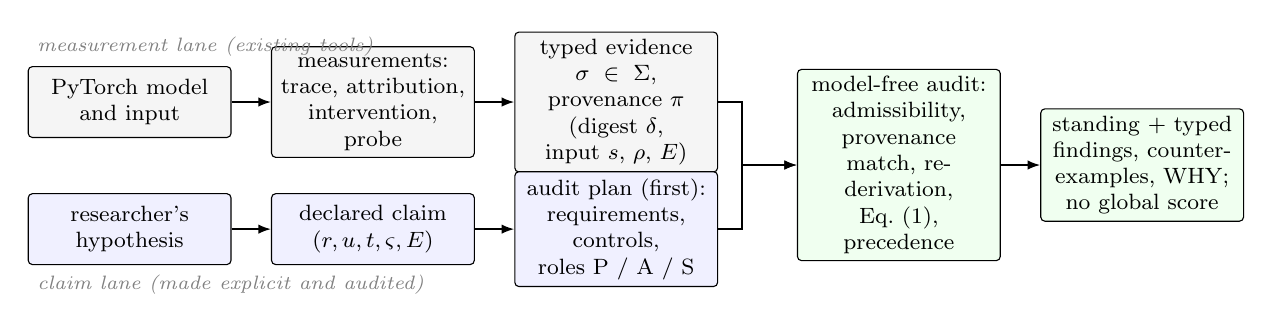
\begin{tikzpicture}[
  font=\footnotesize, node distance=4mm and 5mm,
  box/.style={draw, rounded corners=1.5pt, align=center, minimum height=9mm, inner sep=2.5pt, text width=24mm},
  meas/.style={box, fill=gray!8},
  clm/.style={box, fill=blue!6},
  arr/.style={-{Latex[length=1.6mm]}, semithick}]
\node[meas] (m) {PyTorch model\\and input};
\node[meas, right=of m] (me) {measurements:\\trace, attribution,\\intervention, probe};
\node[meas, right=of me] (ev) {typed evidence\\$\sigma\in\Sigma$, provenance $\pi$\\(digest $\delta$, input $s$, $\rho$, $E$)};
\node[clm, below=7mm of m] (h) {researcher's\\hypothesis};
\node[clm, right=of h] (c) {declared claim\\$(r,u,t,\varsigma,E)$};
\node[clm, right=of c] (p) {audit plan (first):\\requirements, controls,\\roles P / A / S};
\node[box, right=10mm of ev, yshift=-8mm, fill=green!6] (a) {model-free audit:\\admissibility, provenance\\match, re-derivation,\\Eq.~(1), precedence};
\node[box, right=of a, fill=green!6] (o) {standing + typed\\findings, counter-\\examples, WHY;\\no global score};
\draw[arr] (m) -- (me); \draw[arr] (me) -- (ev); \draw[arr] (h) -- (c); \draw[arr] (c) -- (p);
\draw[arr] (ev.east) -- ++(3mm,0) |- (a.west); \draw[arr] (p.east) -- ++(3mm,0) |- (a.west);
\draw[arr] (a) -- (o);
\node[anchor=south west, font=\scriptsize\itshape, text=gray] at (m.north west) {measurement lane (existing tools)};
\node[anchor=north west, font=\scriptsize\itshape, text=gray] at (h.south west) {claim lane (made explicit and audited)};
\end{tikzpicture}
\caption{BeyondNN separates measurements from claims. Measurements become typed, provenance-bound evidence; claims are declared objects; a plan written before the audit states the required evidence, the controls and the role of each configuration. Only \textsc{primary} configurations decide a standing (Proposition~\ref{prop:roles}); the audit re-derives every result from the records and never runs the model.}
\label{fig:pipeline}
\end{figure*}

\begin{figure*}[t]
\centering
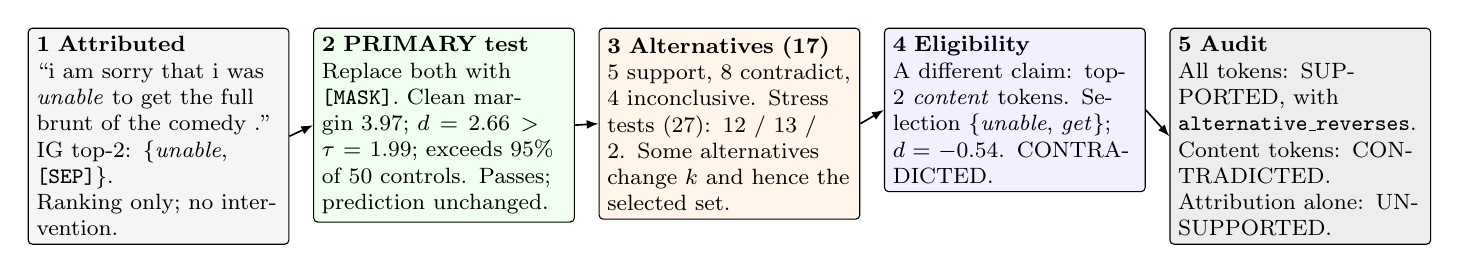
\begin{tikzpicture}[font=\footnotesize, node distance=3mm,
  st/.style={draw, rounded corners=1.5pt, align=left, text width=31mm, minimum height=20mm, inner sep=3pt, anchor=north west},
  arr/.style={-{Latex[length=1.5mm]}, semithick}]
\node[st, fill=gray!8] (s1) at (0,0) {\textbf{1 Attributed}\\ ``i am sorry that i was \textit{unable} to get the full brunt of the comedy .''\\ IG top-2: $\{$\textit{unable}, \texttt{[SEP]}$\}$.\\ Ranking only; no intervention.};
\node[st, fill=green!6, right=of s1.north east, anchor=north west] (s2) {\textbf{2 PRIMARY test}\\ Replace both with \texttt{[MASK]}. Clean margin 3.97; $d=2.66>\tau=1.99$; exceeds 95\% of 50 controls. Passes; prediction unchanged.};
\node[st, fill=orange!8, right=of s2.north east, anchor=north west] (s3) {\textbf{3 Alternatives (17)}\\ 5 support, 8 contradict, 4 inconclusive. Stress tests (27): 12 / 13 / 2. Some alternatives change $k$ and hence the selected set.};
\node[st, fill=blue!6, right=of s3.north east, anchor=north west] (s4) {\textbf{4 Eligibility}\\ A different claim: top-2 \emph{content} tokens. Selection $\{$\textit{unable}, \textit{get}$\}$; $d=-0.54$. CONTRADICTED.};
\node[st, fill=gray!14, right=of s4.north east, anchor=north west] (s5) {\textbf{5 Audit}\\ All tokens: SUPPORTED, with \texttt{alternative\_reverses}.\\ Content tokens: CONTRADICTED.\\ Attribution alone: UNSUPPORTED.};
\foreach \a/\b in {s1/s2,s2/s3,s3/s4,s4/s5} \draw[arr] (\a.east) -- (\b.west);
\end{tikzpicture}
\caption{Running example (BERT-base SST-2, held-out sample 423). Values are read from the per-sample records of the frozen central experiment (\texttt{central775\_D\_heldout\_\{all,content\_tokens\}.json}). \textsc{supported} is scoped to the \textsc{primary} rule and qualified by the alternative finding; the content-token claim concerns a different subject.}
\label{fig:example}
\end{figure*}

\section{Introduction}
\label{sec:intro}

\IEEEPARstart{I}{nterpretability} research increasingly communicates through quantitative artifacts. Attribution methods assign relevance to input features~\cite{simonyan2014saliency,sundararajan2017ig,lundberg2017shap}, probes measure what can be decoded from hidden states~\cite{belinkov2022probing}, activation patching measures what changes when an internal value is replaced~\cite{meng2022rome,zhang2024patching}, and circuit and dictionary methods propose components and features as the units of a mechanism~\cite{wang2023ioi,conmy2023acdc,huben2024sae}. Mature libraries make these artifacts cheap to produce~\cite{kokhlikyan2020captum,nanda2022transformerlens,fiottokaufman2025nnsight,wu2024pyvene,bloom2024saelens}.

An artifact, however, is not the claim that is usually attached to it. Consider a BERT-base sentiment classifier and the held-out sentence ``i am sorry that i was unable to get the full brunt of the comedy .'' IG~\cite{sundararajan2017ig} ranks the word \textit{unable} and the separator token \texttt{[SEP]} highest among its 19 positions. That is a statement about one method, one baseline and one target; it does not establish that the two tokens are necessary for the prediction, which is a question about intervention~\cite{jacovi2020faithfulness,joshi2026causality}. When we intervene, the answer depends on choices. Replacing both tokens with the \texttt{[MASK]} embedding lowers the class margin from 3.97 by 2.66, more than half the clean margin and more than the drop caused by at least 95\% of 50 matched random two-token sets; the predicted class does not change. Eight of the 17 declared alternative configurations contradict this result, and if the claim concerns the two highest-ranked \emph{content} tokens the selection becomes $\{$\textit{unable}, \textit{get}$\}$ and the margin drop is negative (Fig.~\ref{fig:example}).

Conclusions of this kind move when the link between measurement and conclusion changes. Activation-patching results depend on the corruption and the metric~\cite{zhang2024patching}; removal-based faithfulness tests depend on how far the replacement is from the data distribution~\cite{hase2021ood,hooker2019roar}; single-input mediation scores have high variance~\cite{meloux2026variance}; subspace interventions can produce illusory localisation~\cite{makelov2024illusion}; probe accuracy does not show that a model uses what the probe finds~\cite{belinkov2022probing,elazar2021amnesic,hewitt2019control}; and agreement with human rationales is not faithfulness~\cite{jacovi2020faithfulness,deyoung2020eraser}. Recent position papers argue that interpretability claims should be stated with their estimand, intervention class and identification assumptions~\cite{joshi2026causality,lin2026identification}, and call for systems that make the arguments behind claims auditable~\cite{lan2026auditable}. What is missing in practice is an executable link: a representation in which the claim, its units, its replacement, its controls and the alternatives that were tried are explicit enough for a program, not only a reviewer, to check the inference.

We present BeyondNN, an open-source evidence and audit layer for PyTorch~\cite{paszke2019pytorch,roufas2026beyondnn}. BeyondNN is not an attribution, probing or patching method. It records each measurement as typed, provenance-bound evidence, represents claims as declared objects with a relation, a subject, a scope and an eligibility, and re-derives each claim's standing from the recorded evidence under a plan that assigns every configuration a role (\textsc{primary}, \textsc{alternative} or \textsc{stress\_test}). Only \textsc{primary} configurations decide a standing; the others produce typed findings. The audit never runs the model and returns no global score.

The contributions of this paper are:
\begin{enumerate}
\item A formal evidence-audit semantics for interpretability claims about neural networks: typed evidence, provenance, scoped claims with explicit eligibility, a test outcome rule with an attainability condition, configuration roles, admissibility and a precedence rule for standings, with six properties that hold by construction (Section~\ref{sec:framework}).
\item An implementation for PyTorch, released as BeyondNN~0.1.0 (Section~\ref{sec:system}).
\item An evaluation on trained MLP, CNN, BERT-tiny and BERT-base models and on compiled and SIIT-trained transformers with reference mechanisms (Sections~\ref{sec:design}--\ref{sec:results}), including: a fixed-selection decomposition of configuration dependence; a comparison with conventional workflows on identical measurements under injected faults; validation against reference labels that use no intervention on the audited network; replication over independently trained checkpoints; exact re-execution; and the computational cost of the evidence layer.
\end{enumerate}

Throughout, we evaluate claim protocols, not attribution methods. IG is the attribution method in these studies; nothing here shows that IG or attribution in general is unreliable. A \textsc{supported} standing means that the evidence passed the declared \textsc{primary} rule for the stated claim, scope, samples and checkpoint; it is not a statement of logical necessity or of a model's mechanism.

\begin{table*}[t]
\centering
\caption{Built-in, documented capabilities (current releases checked 2026-11-03). ``User'': possible with user code on top of the library. The table positions BeyondNN; it does not rank tools that address different problems.}
\label{tab:capability}
\setlength{\tabcolsep}{3pt}
\footnotesize
\resizebox{\textwidth}{!}{%
\begin{tabular}{lccccccc}
\toprule
capability & Captum & Quantus & causal scrubbing & NNsight / pyvene / TL & CIF & Certified Circuits & BeyondNN \\
\midrule
measurement generation & \checkmark & external & \checkmark & \checkmark & consumes & wraps & partial \\
explicit claim object (relation, subject, scope) & -- & -- & partial (hypothesis) & -- & partial (estimand) & -- & \checkmark \\
evidence-type admissibility & -- & -- & n/a & -- & n/a & -- & \checkmark \\
checkpoint / input provenance per record & user & user & user & user / partial & user & user & \checkmark \\
refusal of mismatched provenance or scope & user & user & user & user & user & user & \checkmark \\
eligibility and estimand matching & -- & -- & partial & -- & \checkmark & -- & \checkmark \\
matched controls as precondition of support & -- & baselines & -- & -- & -- & -- & \checkmark \\
declared alternative configurations with roles & -- & -- & -- & -- & -- & partial & \checkmark \\
per-sample counterevidence retained & -- & scores & aggregate & -- & -- & abstention & \checkmark \\
deterministic re-audit of saved evidence & -- & -- & -- & -- & -- & -- & \checkmark \\
statistical inference / certification & -- & -- & -- & -- & \checkmark & \checkmark & -- \\
\bottomrule
\end{tabular}}
\end{table*}

\begin{table}[t]
\centering
\caption{Evaluation setup. All central studies use correctly classified held-out inputs, one torch thread and CPU execution.}
\label{tab:setup}
\setlength{\tabcolsep}{2.5pt}
\footnotesize
\begin{tabular}{p{0.24\columnwidth}p{0.70\columnwidth}}
\toprule
models & MLP (breast cancer~\cite{wolberg1993breast}; sites input, hidden), CNN (digits~\cite{alpaydin1998digits}; pixels, relu2), BERT-tiny~\cite{turc2019wellread,frantar2021mfac} and BERT-base~\cite{devlin2019bert,morris2020textattack} on SST-2~\cite{socher2013sst,wang2018glue} (token embeddings) \\
held-out samples & 51 / 51 / 60 / 60 / 40 / 40 (302) \\
evidence & G / IG / random top-$k$, $k\in\{5,10,20\}\%$; comprehensiveness and sufficiency; 50 count-matched controls; 3 replacements \\
\textsc{primary} & training mean ([MASK] for BERT), $k$ at 10\%, count null at $q=0.95$, $\tau=0.5\times$ clean margin \\
\textsc{alternative} & resample ([PAD]), $k$ at 5\% and 20\%, magnitude-matched null, $0.5\tau$ \\
\textsc{stress\_test} & zero (MLP input: training minimum), no null, $1.5\tau$ \\
reference models & 8 held-out compiled Tracr programs~\cite{lindner2023tracr} (40 inputs each); 18 SIIT-trained InterpBench transformers~\cite{gupta2024interpbench} (40 inputs each) \\
checkpoints & frozen seed-0 MLP and CNN; seeds 0--4 retrained (Linux); pinned Hugging Face revisions for BERT \\
\bottomrule
\end{tabular}
\end{table}

\section{Related Work}
\label{sec:related}

\paragraph*{Attribution and faithfulness}
Attribution methods~\cite{simonyan2014saliency,sundararajan2017ig,lundberg2017shap} answer ``how relevant is unit $u$ to target $T$ under method $M$ and baseline $B$''. This answer can be insensitive to the model's parameters~\cite{adebayo2018sanity}, sensitive to function-preserving transformations~\cite{kindermans2019unreliability}, and different from attention weights~\cite{jain2019attention,wiegreffe2019notnot}. Jacovi and Goldberg separate plausibility from faithfulness~\cite{jacovi2020faithfulness}; removal tests such as ERASER comprehensiveness and sufficiency~\cite{deyoung2020eraser} and ROAR~\cite{hooker2019roar} operationalise faithfulness and depend on the replacement~\cite{hase2021ood}. In BeyondNN an attribution is \textsc{attributed} evidence and can never decide a causal relation.

\paragraph*{Interventions and causal abstraction}
Causal tracing and activation patching~\cite{meng2022rome,zhang2024patching} estimate how an output depends on a component. Causal scrubbing~\cite{chan2022scrubbing} turns a mechanistic hypothesis into a correspondence with a high-level graph tested by resampling ablations and summarised as recovered loss; causal abstraction~\cite{geiger2025abstraction} unifies patching, mediation and scrubbing, and distributed alignment search~\cite{geiger2024das} aligns high-level variables with representations. Causal scrubbing is the closest methodological precedent to BeyondNN's claim--test structure. BeyondNN differs in scope: it records evidence of several epistemic types from several protocols, keeps alternative interventions as named assumptions with roles, and returns a categorical standing with findings rather than a scalar.

\paragraph*{Probes and concepts}
Decodability does not imply use~\cite{belinkov2022probing}; control tasks~\cite{hewitt2019control} and amnesic probing~\cite{elazar2021amnesic} address this, concept activation vectors~\cite{kim2018tcav} measure sensitivity to a direction, and dictionary features~\cite{huben2024sae,bloom2024saelens} are often given generated labels whose text need not reflect the computation~\cite{turpin2023unfaithful}. BeyondNN keeps decodability, use and labels apart and derives \textsc{validated\_concept} only from passed encoding and use tests.

\paragraph*{Evaluation frameworks, benchmarks and statistics}
Quantus~\cite{hedstrom2023quantus} and OpenXAI~\cite{agarwal2022openxai} score explanation methods; Tracr~\cite{lindner2023tracr}, InterpBench~\cite{gupta2024interpbench}, MIB~\cite{mueller2025mib}, RAVEL~\cite{huang2024ravel} and CausalGym~\cite{arora2024causalgym} provide models or tasks with reference mechanisms. These score methods or proposed mechanisms; BeyondNN audits a particular claim under declared criteria and can itself be evaluated against their references (Section~\ref{sec:res-ref}). Several of these benchmarks define success through interchange interventions, the same family an audit uses, so agreement with them can reflect shared semantics. M\'eloux et al.~\cite{meloux2026variance} show that circuit-discovery estimates are high-variance; Certified Circuits~\cite{anani2026certified} certify the stability of circuit-inclusion decisions under data perturbation; and Certified Interventional Fidelity~\cite{asiaee2026cif} gives anytime-valid confidence sequences for interventional estimands. BeyondNN has none of these inferential guarantees; it records which estimand and assumptions underlie a standing.

\paragraph*{Claims and evidence}
Doshi-Velez and Kim ask that evaluation match the claim~\cite{doshivelez2017rigorous}; Joshi et al. use Pearl's hierarchy to state which claims each kind of evidence can justify~\cite{joshi2026causality}; Lin and Liu propose that causal claims disclose their identification strategy and stress-test its assumptions~\cite{lin2026identification}; and Lan et al. call for expert guidelines and source-based auditing of the arguments that interpretability claims depend on~\cite{lan2026auditable}. We do not claim that matching claims to evidence, or auditing interpretability arguments, is new. Our contribution is narrower: an implemented, machine-checkable semantics that matches typed evidence to scoped claims by provenance, applies declared \textsc{primary} and \textsc{alternative} rules to saved records, and retains counterevidence. Table~\ref{tab:capability} positions it against existing tools.

\paragraph*{Tooling}
Captum~\cite{kokhlikyan2020captum}, TransformerLens~\cite{nanda2022transformerlens}, NNsight~\cite{fiottokaufman2025nnsight}, pyvene~\cite{wu2024pyvene} and SAELens~\cite{bloom2024saelens} produce measurements and perform interventions. BeyondNN complements them: it consumes Captum attributions through an adapter, and its compiled-program study is cross-checked against an independent TransformerLens implementation.

\section{Formal Framework}
\label{sec:framework}

This section defines the objects that BeyondNN represents and the rule by which an audit derives a standing from them. The definitions describe the semantics implemented in BeyondNN~0.1.0; each property in Section~\ref{sec:properties} is stated together with the part of the implementation that enforces it and the test or experiment that checks it. We use one running example: the necessity claim for the Integrated Gradients (IG) selection on held-out sample~423 of a BERT-base sentiment classifier (Fig.~\ref{fig:example}).

\subsection{Evidence and Provenance}

\begin{definition}[Evidence record]
An \emph{evidence record} is a tuple $e=(\mathrm{id},\sigma,v,\pi)$, where $v$ is the recorded value, $\sigma\in\Sigma$ is its epistemic status, $\pi$ is its provenance, and $\mathrm{id}=H(\sigma,v,\pi,\text{references})$ is a content hash. The status set is
$\Sigma=\{$\textsc{observed}, \textsc{measured}, \textsc{attributed}, \textsc{interventional}, \textsc{estimated\_causal}, \textsc{validated\_concept}, \textsc{generated}$\}$.
The status is fixed by the kind of record that produced $e$ and is never supplied by the caller. Statuses are unordered.
\end{definition}

\begin{definition}[Provenance]
The provenance $\pi(e)$ contains the model fingerprint $\delta$ (a digest over the names, dtypes, shapes and bytes of all parameters and persistent buffers), the identity $s=H(x)$ of every input, the target metric $t$, the site, the replacement $\rho$ (name and digest of its value), the declared unit eligibility $E$, the protocol and its version, and the software versions. Two records have the same \emph{conditions} if these fields agree; time and process are recorded but are not part of the conditions.
\end{definition}

In the running example, the IG relevance of the 19 token positions is an \textsc{attributed} record, and the margin change $d=2.66$ obtained by replacing the two selected embeddings with the \texttt{[MASK]} embedding is an \textsc{interventional} record. Both carry the same $\delta$ and the same $s$.

\subsection{Claims, Scope and Eligibility}

\begin{definition}[Claim]
A \emph{claim} is $c=(r,u,t,\varsigma,E)$ with relation $r\in\{$\texttt{necessary\_for}, \texttt{sufficient\_for}, \texttt{increases}, \texttt{decreases}, \texttt{attributed\_to}, \texttt{encodes}$\}$, subject $u$, target $t$, estimand scope $\varsigma\in\{\text{instance},\text{finite\_sample},\text{population}\}$ and eligibility $E$. The subject is either a declared unit set or a \emph{selection rule} $\mathrm{sel}_{M,k}(E)$: the $k$ units of the eligible set $E$ ranked highest by method $M$.
\end{definition}

Eligibility is part of the subject. The claims ``the IG top-2 tokens'' and ``the IG top-2 \emph{content} tokens'' differ even on the same input: in the running example the first selects $\{$\textit{unable}, \texttt{[SEP]}$\}$ and the second $\{$\textit{unable}, \textit{get}$\}$. Changing $k$ also changes the subject whenever the $k$-th and $(k\!+\!1)$-th ranked units differ.

\subsection{Tests, Controls and Outcomes}

\begin{definition}[Necessity test]
Let $m$ be the target metric, $S$ the selected units, $\rho$ the replacement, $\tau$ the effect threshold, $q$ the control criterion and $S_1,\dots,S_J$ random control sets matched to $S$ (by count, or by perturbation magnitude) and drawn from $E$. With $d=m(x)-m(x_{S\leftarrow\rho})$ and $d_j$ the same drop for $S_j$, the test outcome is
\begin{equation}
o=\begin{cases}
\text{inconclusive} & \text{if } x_{S\leftarrow\rho}=x \ \text{(no-op)},\\
\text{supports} & \text{if } d\ge\tau \ \text{and}\ \frac{1}{J}\sum_{j}\mathbb{1}[d_j<d]\ge q,\\
\text{contradicts} & \text{otherwise.}
\end{cases}
\label{eq:test}
\end{equation}
\end{definition}

Control draws identical to $S$ always tie with it and never count as ``below''. When the largest attainable fraction $\bar f=1-|\{j:S_j=S\}|/J$ is smaller than $q$, no model could pass the criterion. The audit then treats a recorded \emph{contradicts} as uninformative and counts it as inconclusive, with the finding \texttt{control\_criterion\_unattainable} (ADR-054); the record itself is not changed. The rank criterion $q$ is a threshold on an empirical fraction over $J$ sampled sets; it is not a calibrated $p$-value. Sufficiency is defined symmetrically by keeping only $S$.

\subsection{Configurations and Roles}

\begin{definition}[Configuration and role]
The \emph{configuration} $\kappa(e)$ of a test result is its value on every assumption axis: replacement, $k$, null (control type and criterion), threshold, method and dataset. A threshold axis value is either the recorded $\tau$ or a declared re-evaluation $\alpha\tau$ applied to the recorded $d$ and $d_j$. An audit plan maps axis values to roles $\{\textsc{primary}<\textsc{alternative}<\textsc{stress\_test}\}$. The role of $\kappa$ is the largest role among its axis values; a configuration with an undeclared value is \textsc{undeclared} and takes no part in the standing.
\end{definition}

In the central experiments every sample is tested under 45 configurations: one \textsc{primary}, 17 \textsc{alternative} and 27 \textsc{stress\_test} (Table~\ref{tab:setup}).

\subsection{Admissibility and Standing}

\begin{definition}[Admissible evidence]
A record $e$ is \emph{admissible} for claim $c$ in plan $P$ if (i) its status is in the set accepted by the relation, $\sigma(e)\in\mathrm{Adm}(r)$, where causal relations accept only \textsc{interventional} and \textsc{estimated\_causal} evidence and \texttt{attributed\_to} accepts \textsc{attributed}; (ii) its estimand scope matches $\varsigma$; (iii) its subject and eligibility match $u$ and $E$; and (iv) its provenance matches $P$: $\delta(e)$ equals the declared checkpoint, and every input identity is a declared sample. Records failing (iv) or an integrity check are excluded and the exclusion is reported.
\end{definition}

\begin{definition}[Standing]
For a claim $c$ and a group $g$ (one sample for instance-scope claims), let $A$ be the admissible results and $A_P\subseteq A$ those in \textsc{primary} configurations. The \emph{standing} is assigned in this order:
(1) \textsc{assumption\_sensitive} if $A_P$ contains both \emph{supports} and \emph{contradicts} and every disagreeing pair differs on a recorded axis, \textsc{mixed} if some pair does not;
(2) \textsc{contradicted} if the verdict derived from $A_P$ under the claim's requirement policy is a contradiction;
(3) \textsc{unsupported} if a finding marks the evidence as the wrong kind, the required controls as missing, or a declared invariance as untested;
(4) \textsc{supported} or \textsc{inconclusive} according to the verdict;
(5) \textsc{not\_evaluated} if $A$ is empty.
\textsc{alternative} and \textsc{stress\_test} configurations whose decisive outcome differs from the \textsc{primary} outcome produce the findings \texttt{alternative\_reverses} (qualifying) and \texttt{stress\_test\_reverses} (informational).
\end{definition}

A standing is a category, not a confidence level, and the audit computes no global score. For per-sample claims there is no claim-level truth value: the report gives the distribution of standings over the declared samples and the identities of counterexamples.

\subsection{Properties}
\label{sec:properties}

The following properties hold by construction of the audit rules. They establish \emph{consistency with the declared semantics}; none of them establishes that a plan, a replacement or a threshold is scientifically appropriate.

\begin{proposition}[Admissibility]
\label{prop:adm}
If no admissible record of $c$ has a status in $\mathrm{Adm}(r)$, the standing of $c$ is neither \textsc{supported} nor \textsc{contradicted}.
\end{proposition}
\emph{Basis.} Condition (i) of admissibility filters records before the verdict is derived. \emph{Checked by:} pre-registered scenarios and code-mutation tests; empirically, every attribution-only audit in this paper (2,480 selection claims) was \textsc{unsupported} (Section~\ref{sec:res-adm}).

\begin{proposition}[Role invariance]
\label{prop:roles}
For a plan with declared roles, the standing of $(c,g)$ is a function of $A_P$ only. Adding, removing or changing \textsc{alternative} or \textsc{stress\_test} results can change the findings but never the standing.
\end{proposition}
\emph{Basis.} The verdict and the disagreement analysis are computed on \textsc{primary} entries only; other roles enter only the finding generator. \emph{Checked by:} all 47 held-out samples with \texttt{alternative\_reverses} retain the standing \textsc{supported} (Section~\ref{sec:res-config}).

\begin{proposition}[Monotone reversal count]
\label{prop:mono}
The number of groups carrying \texttt{alternative\_reverses} is non-decreasing in the set of declared \textsc{alternative} configurations.
\end{proposition}
\emph{Basis.} The finding is an existential statement over the declared alternatives. Consequently, an at-least-one reversal count measures dependence on a declared test family; it is not an instability rate.

\begin{proposition}[Threshold asymmetry]
\label{prop:thr}
With $d$, $d_j$ and $q$ fixed, re-evaluating~\eqref{eq:test} at $\alpha\tau$ with $\alpha<1$ cannot turn \emph{supports} into \emph{contradicts}, and $\alpha>1$ cannot turn \emph{contradicts} into \emph{supports}.
\end{proposition}
\emph{Basis.} The outcome is monotone in $\tau$. \emph{Checked by:} in every re-run reported here, the $\tau\times0.5$ alternative reversed no supported claim (Table~\ref{tab:decomp}).

\begin{proposition}[Provenance refusal]
\label{prop:prov}
A result whose model fingerprint or input identity is not declared in the plan never contributes to a standing. A declared group without admissible evidence is \textsc{not\_evaluated}.
\end{proposition}
\emph{Basis.} Condition (iv) of admissibility. \emph{Checked by:} the injected wrong-checkpoint and wrong-input faults of Section~\ref{sec:res-cmp} (5/5 \textsc{not\_evaluated} each).

\begin{proposition}[Re-derivability]
\label{prop:det}
The audit is a deterministic function of the evidence records, the plan and the audit-semantics version. A stored report can be re-derived from saved evidence without the model, and any edit to a stored record changes its content hash and is rejected on load.
\end{proposition}
\emph{Basis.} Content-addressed records and a model-free audit. \emph{Checked by:} re-audits from disk identical to in-memory reports, and rejection of every tampered trace (Sections~\ref{sec:res-cmp} and~\ref{sec:res-repro}).

\section{Implementation}
\label{sec:system}

BeyondNN~0.1.0 is a Python library for PyTorch released under the Apache-2.0 licence (\texttt{pip install beyondnn}; source at \url{https://github.com/NikolasRoufas/beyondnn}). It has 75 modules, is tested on Python 3.10, 3.12 and 3.14 with PyTorch~$\ge$2.3, and \texttt{import beyondnn} does not import PyTorch. We describe only what the evaluation uses; all names are public API.

\paragraph*{Layers}
\texttt{core} handles tracing, hooks, sites, sample identity and persistence; \texttt{schema} and \texttt{provenance} hold the immutable, versioned records, statuses, claims and model fingerprints. Five modules produce or assess evidence: \texttt{attribution}, \texttt{interventions}, \texttt{faithfulness}, \texttt{concepts} and \texttt{audits}. \texttt{explain} composes the structured WHY. Every layer below \texttt{audits} produces records; the audit only reads them. Each record kind is versioned and older versions are migrated on load.

\paragraph*{Instrumentation}
\texttt{bnn.trace(model, x, sites=...)} runs one forward pass and returns a trace; hooks exist only during a recording, and the user's model is never modified. Tracing refuses situations in which a record could be silently wrong (foreign forward hooks, models spread over several devices, structural changes during recording).

\paragraph*{Evidence producers}
\texttt{bnn.attribute} records \textsc{attributed} evidence (native gradient, input$\times$gradient and IG; Captum methods through an optional adapter, verified with Captum~0.9). \texttt{bnn.intervene} records \textsc{interventional} effects of the declared operations \texttt{zero}, \texttt{constant}, \texttt{patch} and \texttt{direction} on sites, units or feature directions. The \texttt{faithfulness} module implements selection-based tests: \texttt{F.top\_k} turns an attribution into a selection (descending absolute score, ties broken by index, optionally among declared eligible units), \texttt{F.comprehensiveness} and \texttt{F.sufficiency} declare the test of~\eqref{eq:test}, \texttt{F.replacement} declares a named replacement tensor (for example a training mean, a resampled activation or a \texttt{[MASK]} embedding), and \texttt{F.controls} declares matched random controls with a recorded seed. There is no implicit zero replacement.

\paragraph*{Plans, audits and persistence}
An audit plan is itself a content-addressed record. It declares the checkpoint, the samples, the claims, each claim's requirement (assessment policy, whether controls are mandatory, alternative threshold criteria), the invariances the claim asserts, the configuration roles and counterexample caps. \texttt{bnn.audit(evidence, plan=plan)} returns a deterministic report with sorted keys that embeds the plan, a digest of the evidence identifiers and its producer (BeyondNN version and audit-semantics version). \texttt{AU.save\_evidence} and \texttt{AU.load\_evidence} save and reload exactly the traces an audit ingests, with full re-validation; \texttt{AU.verify\_report(report, evidence, plan)} re-derives a stored report and raises an error on any difference. Concept evidence follows the same pattern: an encoding test against random directions and label permutations, and a use test that removes the concept direction and compares the target change with a declared minimum in the target's own scale.

\section{Evaluation Design}
\label{sec:design}

We ask whether making claims explicit changes what can be concluded, and how the audit rules behave against reference mechanisms and conventional workflows. Seven research questions organise the evaluation:
\textbf{RQ1} How often, and through which assumption, do declared alternatives reverse a \textsc{primary} conclusion?
\textbf{RQ2} Does attribution evidence establish necessity, and is inadmissible evidence refused?
\textbf{RQ3} Which workflow errors does the audit detect, compared with conventional workflows on the same measurements?
\textbf{RQ4} How do \textsc{primary} standings relate to reference labels that are not defined by the audited intervention?
\textbf{RQ5} Does concept validation separate decodability from use?
\textbf{RQ6} Are the central findings stable across independently trained checkpoints?
\textbf{RQ7} Can studies be re-executed and re-audited exactly, and what does the evidence layer cost?

\paragraph*{Setup}
Table~\ref{tab:setup} summarises models, sites, samples and configurations. Central held-out inputs are correctly classified inputs drawn in seeded order after the development samples, so all central results are conditional on correct prediction. We test necessity and sufficiency of IG, gradient and random top-$k$ selections against the predicted-class margin.

\paragraph*{Protocols and blinding}
Each original held-out round had a plan frozen before it ran (Phase~7.5 and~7.75 plans in the repository). Later protocol revisions (ADR-053 on eligibility and ADR-054 on attainability) were informed by earlier results, so the work is not uniformly blind: the central 47/52 is a re-audit of held-out samples whose earlier audit had given 49/52. Every experiment new to this paper (Stages~2--4) had a protocol committed before execution, stating hypotheses, units, budgets and stopping rules; one baseline implementation error found during execution is reported in Section~\ref{sec:res-cmp}.

\paragraph*{Units and statistics}
The observational unit is a (site, held-out sample) pair for central claims and a (component, input) instance for reference models. Counts are exact. Wilson and input-level bootstrap intervals are descriptive and unclustered: instances share components and programs, and samples share checkpoints. Between-checkpoint spread is reported directly (RQ6). No interval here quantifies uncertainty over new models.

\section{Results}
\label{sec:results}

\subsection{RQ1: Configuration Dependence, Decomposed}
\label{sec:res-config}

On the six central sites, IG necessity was \textsc{primary}-supported on 52 of 302 held-out samples, and on 47 of these at least one declared \textsc{alternative} configuration contradicted the \textsc{primary} result. The committed per-sample records store only role-by-outcome counts, and their recorded reversal axes merge \textsc{alternative} and \textsc{stress\_test} findings, so they cannot attribute reversals to assumptions. We therefore re-ran the frozen central design unchanged, exporting every tested configuration with its axis values. Using the frozen macOS checkpoints on a Linux x86-64 server, the re-run reproduced every per-sample standing, finding code and outcome profile of the frozen results (\ReproDiffs{} differences over all six sites and six claims).

Table~\ref{tab:decomp} and Fig.~\ref{fig:decomp} decompose the reversals. A configuration that keeps $k$ keeps the selected units, because the IG ranking does not depend on the replacement, null or threshold; a configuration that changes $k$ changes the claim's subject. Of the \TotRev{} reversed samples, \TotFixed{} were reversed by an alternative that keeps the selected units fixed, and \TotKOnly{} only by alternatives that change $k$. Changing only the replacement reversed \TotRepl{} samples and changing only the null (count- to magnitude-matched controls) \TotNull{}; no reversal required a combination of axes without a single-axis explanation. The halved threshold reversed none of the supported claims, as Proposition~\ref{prop:thr} requires. The split differs by model: on the CNN pixel site \CnnFixed{} of \CnnRev{} reversals hold the units fixed, whereas on BERT-tiny only \TinyFixed{} of \TinyRev{} do and \TinyKOnly{} arise only from a change of $k$. All reversed samples retain the standing \textsc{supported} with the qualifying finding \texttt{alternative\_reverses} (Proposition~\ref{prop:roles}).

These counts are conditional on the declared family (Proposition~\ref{prop:mono}) and are not instability rates. They separate two readings that the aggregate 47/52 conflated: dependence of a \emph{fixed} claim on the intervention or control rule, and dependence of the \emph{claim itself} on the selection size.

\begin{table}[t]
\centering
\caption{Decomposition of ALTERNATIVE reversals of PRIMARY-supported IG necessity claims (re-run of the frozen central design, held-out samples). \emph{Any}: $\ge 1$ ALTERNATIVE configuration contradicts. \emph{Fixed}: a contradicting ALTERNATIVE keeps $k$, hence the selected units. Single-axis columns: contradiction by a configuration that differs from PRIMARY only on that axis. \emph{$k$ only}: reversed only by configurations that change $k$. Counts per sample; samples are nested in four checkpoints.}
\label{tab:decomp}
\setlength{\tabcolsep}{2.6pt}
\footnotesize
\resizebox{\columnwidth}{!}{%
\begin{tabular}{lrrrrrrrrr}
\toprule
 & & & \multicolumn{2}{c}{reversed} & \multicolumn{4}{c}{single-axis reversal} & \\
\cmidrule(lr){4-5}\cmidrule(lr){6-9}
site & $n$ & sup. & any & fixed & repl. & null & thr. & $k$ & $k$ only \\
\midrule
MLP input & 51 & 8 & 7 & 3 & 3 & 1 & 0 & 5 & 4 \\
MLP hidden & 51 & 4 & 2 & 2 & 2 & 0 & 0 & 2 & 0 \\
CNN pixels & 60 & 14 & 13 & 10 & 9 & 7 & 0 & 7 & 3 \\
CNN relu2 & 60 & 1 & 1 & 1 & 1 & 0 & 0 & 1 & 0 \\
BERT-tiny & 40 & 14 & 13 & 3 & 0 & 3 & 0 & 11 & 10 \\
BERT-base & 40 & 11 & 11 & 4 & 4 & 1 & 0 & 10 & 7 \\
\midrule
Total & 302 & 52 & 47 & 23 & 19 & 12 & 0 & 36 & 24 \\
\midrule
\multicolumn{10}{l}{\emph{fresh, never-inspected samples (protocol P3)}} \\
CNN pixels & 60 & 19 & 19 & 16 & 10 & 12 & 0 & 15 & 3 \\
CNN relu2 & 60 & 2 & 2 & 1 & 1 & 0 & 0 & 1 & 1 \\
BERT-tiny & 40 & 9 & 6 & 1 & 0 & 1 & 0 & 4 & 5 \\
\bottomrule
\end{tabular}}
\end{table}


\begin{figure}[t]
\centering
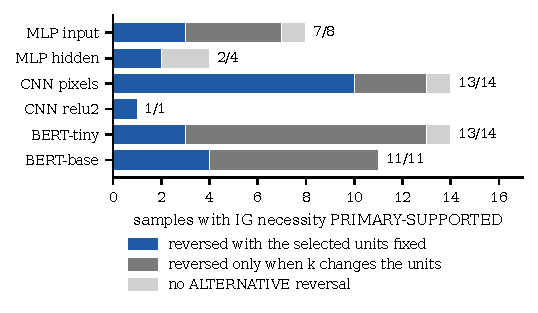
\includegraphics[width=\columnwidth]{figures/fig_decomposition.pdf}
\caption{ALTERNATIVE reversals of PRIMARY-supported IG necessity claims by source (re-run of the frozen design; Table~\ref{tab:decomp}). Counts per held-out sample.}
\label{fig:decomp}
\end{figure}

\subsection{RQ2: Attribution, Necessity and Admissibility}
\label{sec:res-adm}

On BERT-base, IG's \textsc{primary} selection contained \texttt{[SEP]} or \texttt{[CLS]} on 30 of 40 samples, and \texttt{[SEP]} on 10 of the 11 samples where necessity was supported. Declaring the claim the analyst usually intends, about the top-$k$ \emph{content} tokens with $k$, rankings and controls computed over content tokens only, gave 6 of 40 supports [0.07, 0.29]. Only 3 of the 11 all-token supports survived; 5 became \textsc{contradicted} and 3 \textsc{inconclusive} (a single content token leaves the control criterion unattainable), and 3 samples became newly supported. The special-token pattern was known from an earlier round before the content-token claim was declared. By the admissibility rule, attribution-only evidence never supported an intervention claim: all 2,480 attribution-only selection claims in this work (280 central, 1,960 InterpBench, 240 Tracr) were \textsc{unsupported} with \texttt{attribution\_is\_not\_intervention} (Proposition~\ref{prop:adm}). This is a consequence of the type rule, not empirical evidence that attribution is unreliable.

\subsection{RQ3: Comparison with Conventional Workflows}
\label{sec:res-cmp}

To test what the audit adds, we compared it with conventional workflows on \emph{identical} measurements: the frozen central evidence for 20 held-out MLP samples, logged as a careful researcher would (checkpoint and input hashes, configuration, drops, control drops, outcome). B0 reports the \textsc{primary} outcome; B1 adds \BOneLoc{} lines of checks written for this study (checkpoint, input, intervention present, controls present, $k$, outcome recomputation, and a multiverse rule); BeyondNN audits with the frozen plan (\PlanLoc{} lines, reused unchanged). We injected seven faults into both representations (Table~\ref{tab:cmp}). A first run used a baseline that ranked IG scores by signed rather than absolute value; after correcting it to the library's rule, the baseline and BeyondNN selected identical units and reached identical outcomes on 20 of 20 samples (largest drop difference $2.9\times10^{-6}$).

Single-configuration reporting surfaced none of the faults and would have reported 37 erroneous \textsc{supported} conclusions. The careful checker detected every fault, but only through a check written for that fault. The audit detected every fault from its declared plan without fault-specific code and with no false alert on unaffected samples. The two differed in two respects. B1's multiverse rule flagged one additional sample whose only contradicting alternative had an unattainable control criterion; the flat log records it as a contradiction, whereas the audit treats it as uninformative. And B1 localised tampered outcomes to the sample, whereas BeyondNN refused the whole evidence set because the edited record no longer matched its content hash. The result is therefore not that the audit detects errors a careful researcher cannot, but that its checks are part of the representation, apply to any plan, and encode edge cases (attainability, eligibility, provenance) that hand-written checks must anticipate. By lines of code it was not cheaper in this study.

\begin{table}[t]
\centering
\caption{Injected workflow faults on identical measurements (MLP, 20 held-out samples). Detected/affected, false alerts in parentheses. B0: single-configuration report. B1: conventional log with 54 lines of fault-specific checks. BeyondNN: the frozen plan, no fault-specific code. $^\ast$Study-level refusal: the edited trace fails its content hash and the evidence set is not loaded.}
\label{tab:cmp}
\setlength{\tabcolsep}{2.4pt}
\footnotesize
\resizebox{\columnwidth}{!}{%
\begin{tabular}{lrrrrr}
\toprule
fault & aff. & wrong sup. & B0 & B1 & BeyondNN \\
\midrule
F1 attribution as necessity & 20 & 20 & 0 & 20/20 (0) & 20/20 (0) \\
F2 wrong checkpoint & 5 & 1 & 0 & 5/5 (0) & 5/5 (0) \\
F3 wrong input & 5 & 0 & 0 & 5/5 (0) & 5/5 (0) \\
F4 wrong selection size & 5 & 1 & 0 & 5/5 (0) & 5/5 (0) \\
F5 omitted controls & 20 & 6 & 0 & 20/20 (0) & 20/20 (0) \\
F6 configuration dependence & 4 & 4 & 0 & 4/4 (1) & 4/4 (0) \\
F7 tampered outcome & 5 & 5 & 0 & 5/5 (0) & 5/5$^\ast$ (--) \\
\bottomrule
\end{tabular}}
\end{table}


\subsection{RQ4: Reference Labels Not Defined by the Audited Intervention}
\label{sec:res-ref}

\paragraph*{Compiled programs}
Eight held-out Tracr programs~\cite{lindner2023tracr} label each component by whether its variable is read by the output expression, independently of any intervention; the labels describe structural use, not per-input necessity. The \textsc{primary} resample test supported 0 of 400 decoy component--input tests (95\% Wilson upper bound 0.95\%), including 0 of 57 IG-selected decoy heads, and 591 of 760 tests of used components (77.8\% [74.7, 80.6]); each of the 19 used components passed on 28--38 of its 40 inputs and each of the 10 decoys on none. Two programs contain decoys correlated with the used variable: 0 of their 160 decoy tests were supported, of which 80 test an exact copy of the used variable. The 169 contradicted tests of used components are inputs on which the sampled counterfactual left the relevant value unchanged; an independent TransformerLens interchange agreed with the \textsc{primary} outcome on all 1,160 decisive instances. Mean replacement behaved similarly (0/400; 586/760), whereas zero replacement, a \textsc{stress\_test}, met the support rule for all 400 decoy and 760 used tests, because zero is not a valid one-hot value (Fig.~\ref{fig:reference}a).

\paragraph*{Trained transformers}
InterpBench's 18 held-out SIIT-trained transformers~\cite{gupta2024interpbench} were previously scored against labels filtered by the trained models' own resample ablations, which makes agreement partly circular. We re-scored the committed standings against \emph{specification} labels that use no intervention on the trained network: a node--input instance is necessary if the node is in the benchmark circuit and interchanging the corresponding node of the compiled high-level program changes that program's output. The \textsc{primary} test supported \IbTp{} of \IbPos{} specification-necessary instances and \IbFp{} of \IbNeg{} specification-unnecessary instances (\IbFpPct\%); zero replacement supported \IbZeroFp{} (\IbZeroFpPct\%) of the latter (Fig.~\ref{fig:reference}b). All \IbFp{} disagreements are non-circuit nodes, 17 of them in one model, on which the trained network's own resample ablation flips its prediction: the network does not implement its specification exactly there, and the audit reports the network, not the specification. This re-analysis was performed after the earlier results were known, and SIIT training itself uses interchange interventions, so the labels are independent of the audited evaluation but not of the intervention family that shaped the networks.

\begin{figure}[t]
\centering
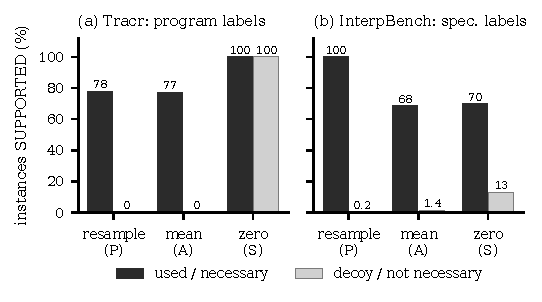
\includegraphics[width=\columnwidth]{figures/fig_reference.pdf}
\caption{Each configuration evaluated as if it were the only one, against reference labels not defined by the audited intervention: (a) program-defined structural labels of 8 compiled Tracr programs; (b) specification labels of 18 SIIT-trained InterpBench transformers. Percentages of instances supported; unclustered.}
\label{fig:reference}
\end{figure}

\subsection{RQ5: Decodability versus Use}

Four held-out numeric Tracr programs each contain a used indicator (K+), a decoy indicator read with coefficient exactly zero (K$-$) and a permuted-label control (K0). The encoding test supported K$-$ in all four programs, so decodability did not separate the variables; the use test did. Removing the K+ direction changed the target by 0.16--0.30, above the declared scale-relative minimum (0.2 standard deviations of the training target, ADR-055), and removing K$-$ changed it by exactly zero. All 4 K+ concepts were validated and none of the 8 K$-$ or K0 concepts under either threshold rule. The held-out programs did not discriminate between the scale-relative and an absolute threshold; on a constructed grid (6 use weights $\times$ 5 output scales) the absolute rule changed its verdict with the output scale in both directions while the relative rule validated exactly the weights $\ge 0.5$ at every scale. The relative rule was adopted after an absolute rule had failed to validate a known-used Tracr variable (use effect 0.06 against 0.1); no concept in a trained network has independent truth here.

\subsection{RQ6: Independently Trained Checkpoints}
\label{sec:res-seeds}

All central findings above rest on one checkpoint per model. We retrained the MLP and CNN with five seeds and re-ran the full central design on each checkpoint's held-out samples (Table~\ref{tab:seeds}, Fig.~\ref{fig:seeds}). Two hypotheses stated before the runs held on every checkpoint and site: IG necessity support exceeded random-selection support, and wherever at least three IG claims were supported, at least half carried an \textsc{alternative} reversal (75--100\%). The fixed-subject share replicated on the CNN pixel site (10--15 of 12--22 supports, 60--83\%). Absolute counts varied: IG supports on CNN pixels ranged from 12 to 22 of 60, so a single-checkpoint count is not a stable model-class estimate. On the CNN relu2 site, every IG necessity test carried \texttt{control\_criterion\_unattainable} on every checkpoint, so its few supports come from the remaining decisive tests. Gradient top-$k$ was supported on 37--41 of 60 CNN pixel samples on every checkpoint, against 12--22 for IG. The same code and seed produced different checkpoint digests on Linux and macOS; on these checkpoints the central counts were nevertheless identical. The BERT models have one checkpoint each.

\begin{table}[t]
\centering
\caption{Independently trained checkpoints (Linux x86-64; seeds 0--4) and the frozen macOS checkpoint. Each cell: IG necessity PRIMARY-supported / of which ALTERNATIVE-reversed / random selection supported, out of 51 (MLP) or 60 (CNN) held-out samples drawn by the same rule per checkpoint.}
\label{tab:seeds}
\setlength{\tabcolsep}{2.2pt}
\footnotesize
\resizebox{\columnwidth}{!}{%
\begin{tabular}{lcccccc}
\toprule
site & frozen & seed 0 & seed 1 & seed 2 & seed 3 & seed 4 \\
\midrule
MLP input & 8/7/1 & 8/7/1 & 8/8/0 & 7/6/0 & 4/4/1 & 7/6/1 \\
MLP hidden & 4/2/0 & 4/2/0 & 2/1/0 & 2/2/0 & 2/2/0 & 2/2/0 \\
CNN pixels & 14/13/1 & 14/13/1 & 22/20/2 & 20/19/3 & 17/16/0 & 12/12/1 \\
CNN relu2 & 1/1/0 & 1/1/0 & 2/1/1 & 3/3/1 & 4/3/0 & 4/3/0 \\
\bottomrule
\end{tabular}}
\end{table}


\begin{figure}[t]
\centering
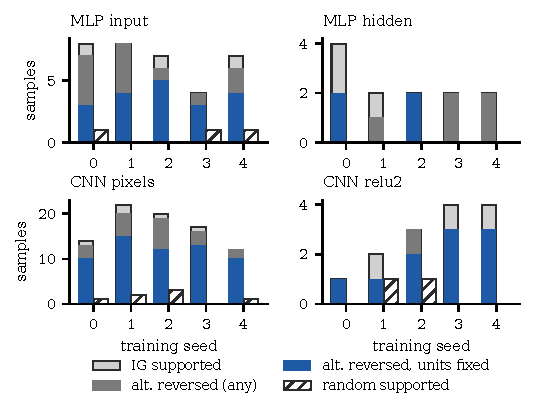
\includegraphics[width=\columnwidth]{figures/fig_seeds.pdf}
\caption{Central findings on five independently trained checkpoints per model (Table~\ref{tab:seeds}). Held-out sets are drawn by the same rule per checkpoint and differ between checkpoints.}
\label{fig:seeds}
\end{figure}

\subsection{RQ7: Re-execution, Re-audit and Cost}
\label{sec:res-repro}

\paragraph*{Re-execution}
Re-running the frozen central design from source on a different platform reproduced every per-sample audit output of the four central models (RQ1). For the MLP, evidence saved to disk (1.7 and 2.0~GB per site), reloaded in the same run and re-audited gave reports identical to the in-memory ones, and \texttt{verify\_report} re-derived each saved report from disk. Every tampered trace was refused on load (RQ3).

\paragraph*{Cost}
Table~\ref{tab:cost} and Fig.~\ref{fig:cost} separate evidence generation from the model-free audit. The audit and its verification are independent of the model, so their share falls as models grow: about a third of the total for the MLP and CNN sites and a few percent for the BERT models. At the level of one test, the evidence layer is not free: one \textsc{primary} IG necessity test with 50 controls on the 30-feature MLP took \CostBnnMs{}~ms through BeyondNN and \CostPlainMs{}~ms in plain PyTorch with Captum, about \CostRatio{} times longer, because record construction, hashing and provenance dominate the computation of so small a model. Saved evidence is large when every control effect is retained (33--39~MB per MLP sample).

\begin{table}[t]
\centering
\caption{Cost per held-out sample of the full central design (one CPU thread, Linux x86-64). Evidence: model execution and BeyondNN record construction for all results of the sample. Audit and verify: model-free. Share: audit + verify as \% of the total. Report: size of the site's report (MB). RSS: peak resident memory of one process (MB).}
\label{tab:cost}
\setlength{\tabcolsep}{2.2pt}
\footnotesize
\resizebox{\columnwidth}{!}{%
\begin{tabular}{lrrrrrrrr}
\toprule
site & $n$ & res. & evid. (s) & audit (s) & verify (s) & share & report & RSS \\
\midrule
MLP input & 51 & 72 & 3.7 & 0.967 & 1.154 & 36.7 & 20.3 & 5906 \\
MLP hidden & 51 & 72 & 4.4 & 1.033 & 1.206 & 33.7 & 20.0 & 6866 \\
CNN pixels & 60 & 72 & 3.7 & 1.132 & 1.181 & 38.8 & 23.9 & 3364 \\
CNN relu2 & 60 & 72 & 4.3 & 1.099 & 1.025 & 33.2 & 23.6 & 3836 \\
BERT-tiny & 40 & 69 & 70.4 & 1.211 & 1.105 & 3.2 & 15.4 & 1427 \\
\bottomrule
\end{tabular}}
\end{table}


\begin{figure}[t]
\centering
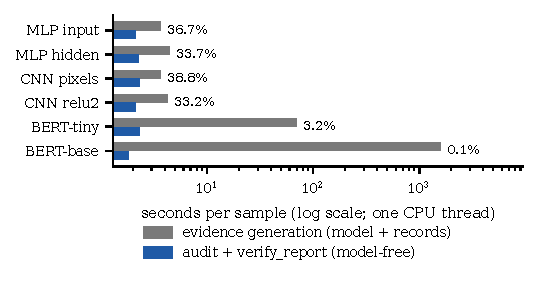
\includegraphics[width=\columnwidth]{figures/fig_cost.pdf}
\caption{Cost per held-out sample of the full central design: evidence generation (model execution and record construction) versus the model-free audit and verification; labels give the audit share. One CPU thread, Linux x86-64.}
\label{fig:cost}
\end{figure}

\subsection{Case Study: Plausibility versus Necessity on e-SNLI}

On 40 held-out e-SNLI samples~\cite{camburu2018esnli,bowman2015snli}, with BERT-base fine-tuned on SNLI, we compared three equal-size token selections: annotator~1's rationale, IG's top-$k$ and a random set, each tested for necessity with the \texttt{[MASK]} replacement and matched controls. IG overlapped more with the human rationale than random sets did (token F1 0.34 [0.26, 0.42]; IG minus random $+0.149$, Bonferroni 98.75\% [0.031, 0.270]), yet necessity was supported for the human rationale on 10, for IG on 7 and for random sets on 3 of 40 samples, opposite to the directional prediction; the paired IG-minus-human difference was $-0.075$ [$-0.225$, 0.075], so no population difference is established. On 17 of the 40 samples the model predicts the same label with an empty premise (empty-premise accuracy 0.456 against chance 1/3~\cite{gururangan2018artifacts}), and 5 of IG's 7 supports fall in that stratum (exploratory). Human rationales are plausibility references, not causal ground truth; one annotator, one model and 40 samples limit this study.

\section{Limitations}
\label{sec:limits}

\paragraph*{What a standing means}
\textsc{supported} means that the \textsc{primary} evidence met the declared rule for the stated claim, scope, samples and checkpoint; it is neither a universal truth value nor a population claim, and \textsc{unsupported} and \textsc{inconclusive} are refusals, not refutations. The properties of Section~\ref{sec:properties} establish consistency with the implemented semantics. They do not establish that a plan, replacement, threshold or control is scientifically adequate, and evidence produced by a flawed protocol is re-derived faithfully by the same code. A plan cannot reveal alternatives that were never declared, and the at-least-one reversal count grows with the declared family (Proposition~\ref{prop:mono}).

\paragraph*{Reference truth}
Program-defined labels exist only for small compiled programs (one or two layers, at most three heads, one-hot or numeric variables), and they mark structural use, not per-input necessity. The specification labels of the SIIT-trained InterpBench models use no intervention on the trained network, but SIIT training itself uses interchange interventions, so the labels are independent of the audited evaluation and not of the intervention family that shaped the networks. No central model (MLP, CNN, BERT) has independent mechanism truth, and the InterpBench re-analysis was performed after the Phase-7.5 results were known.

\paragraph*{Protocol dependence and blinding}
Researchers choose the \textsc{primary} configuration, alternatives, thresholds and controls. Each held-out round had a frozen plan, but plans were revised after earlier results (ADR-053/054); the reported 47/52 is a re-audit of samples whose earlier audit (49/52) had been seen. The 169 contradicted tests of structurally used Tracr components are single-counterfactual non-changes, not false negatives against per-input labels; multiple counterfactual draws would address this at higher evidence cost.

\paragraph*{Statistics and replication}
Wilson and bootstrap intervals are descriptive and unclustered: instances share programs, inputs share checkpoints. The MLP and CNN results were replicated over five independently trained checkpoints; BERT-tiny and BERT-base each have one checkpoint. Nothing here supports generalisation to new architectures or scales; the largest model is BERT-base (110M parameters) on CPU.

\paragraph*{Comparison and cost}
The comparative study uses faults designed by the authors and a conventional checker written knowing them; it measures which checks exist by default, not how often researchers err. On a 30-feature MLP the evidence layer made one test about 23 times slower than plain PyTorch; its share of total cost shrinks with model size (Table~\ref{tab:cost}), but for very small models it dominates. Hooks observe only instrumented module boundaries, and model fingerprints cover parameters and persistent buffers, not Python source or undeclared constructor settings.

\section{Conclusion}
\label{sec:conclusion}

Between an interpretability measurement and the conclusion drawn from it lies a claim with a relation, a scope, a set of units, a replacement, a control and a threshold. BeyondNN makes that claim the object of analysis: evidence carries its epistemic status and provenance, claims are declared objects, configurations have declared roles, and audits re-derive every standing from recorded evidence without a global score. On trained MLP, CNN and BERT models, most \textsc{primary}-supported IG necessity claims carried a qualifying reversal; with the selected units held fixed, the replacement and the control rule alone reversed many of them, while on the token models most reversals came only from changes of the selection size, that is, of the claim's subject. Against program-defined and specification labels, the \textsc{primary} test supported no decoy and almost no specification-excluded node, and the exceptions were nodes the trained network demonstrably uses. On identical measurements, the audit surfaced every injected workflow fault without fault-specific code, which a careful conventional checker matched only with checks written for each fault. BeyondNN does not determine what a model computes and cannot supply evidence that was never recorded; it makes interpretability claims explicit, testable, provenance-aware and reproducible, and makes claims that the evidence does not support easier to reject.

\section*{Code and Data Availability}
BeyondNN~0.1.0, all experiment scripts, frozen plans and committed per-sample results are available at \url{https://github.com/NikolasRoufas/beyondnn}; the revision experiments of this paper are in \path{experiments/tnnls_revision/}, with protocols in \path{docs/tnnls_revision/protocols/} and a claim-to-source table in \path{docs/tnnls_revision/RESULT_SOURCE_TRACEABILITY.csv}.

\section*{Acknowledgment}
\emph{[AI-assistance disclosure for author review, following the IEEE Author Guidelines for AI-generated text.]} An AI coding assistant (Claude Code, Anthropic) was used in the revision of this article: to write analysis and experiment scripts (Section~\ref{sec:results}; repository directory \path{experiments/tnnls_revision/}), to recompute reported values from committed artifacts, and to draft and edit the text of all sections and the figure and table generation code. All experiments, numbers and references were checked against the repository's artifacts; the authors reviewed and take responsibility for the content.


\bibliographystyle{IEEEtran}
\bibliography{refs}

\end{document}
